\documentclass[a4paper,10pt]{article}

\usepackage[utf8]{inputenc}

\usepackage[margin=1.2in]{geometry}
\usepackage{parskip}

\usepackage{amsmath}
\usepackage{amssymb}

\usepackage{graphicx}
\usepackage{float}

\usepackage{listings}
\usepackage[dvipsnames]{xcolor}
\definecolor{lightgray}{gray}{0.97}

\lstset{  
    backgroundcolor=\color{lightgray},   
    commentstyle=\color{gray},
    keywordstyle=\color{magenta},
    numberstyle=\tiny\color{cyan},
    stringstyle=\color{OliveGreen},
    frame=top,frame=bottom,
    basicstyle=\small\normalfont\sffamily,
    stepnumber=1,
    numbersep=10pt,
    tabsize=4,
    extendedchars=true,
    breaklines=true,
    captionpos=t,
    mathescape=true,
    showspaces=false,
    showtabs=false,
    xleftmargin=17pt,
    framexleftmargin=17pt,
    framexrightmargin=17pt,
    framexbottommargin=5pt,
    framextopmargin=5pt,
    showstringspaces=false
}


\title{Numerical Recipes in Astrophysics \\
        \large Assignment 1}
\author{Brendon Walter (s2078864)}


\begin{document}

    \maketitle

    \begin{abstract}
        In this first assignment for Numerical Recipes in Astrophysics (taught by Dr. Marcel van Daalen at Leiden University, Spring 2019), we use the algorithms learned in the first half of the course to ....
    \end{abstract}

    \tableofcontents

    \newpage
\section{Routines}

    \subsection{Poisson Distribution}
        
        \begin{equation}
            P(k) = \frac{\mu^k e^{-\mu}}{k!}
            \label{eq:poisson}
        \end{equation}

        \lstinputlisting[language=Python, caption=poisson.py]{poisson.py}
        \lstinputlisting[language=Python]{output/poisson.txt}
        
        
    \newpage
    \subsection{Random Number Generator}
    
        \begin{equation}
            x_{j+1} = a x_{j} + c \mod m
            \label{eq:mlcg}
        \end{equation}
        
        \begin{equation}
            \begin{array}{l}
            x_{j+1} = x_{j} \land (x_{j} \ll a) \\
            x_{j+1} = x_{j} \land (x_{j} \gg b) \\
            x_{j+1} = x_{j} \land (x_{j} \ll c)
            \end{array}
            \label{eq:xor_shift}
        \end{equation}

        \lstinputlisting[language=Python, caption=RNG.py]{RNG.py}
        \lstinputlisting[language=Python]{output/RNG.txt}
        
        \begin{figure}[H]
            \centering
            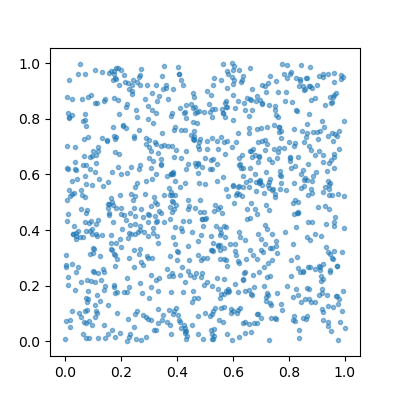
\includegraphics[height=6cm]{output/RNG_scatter.png}
            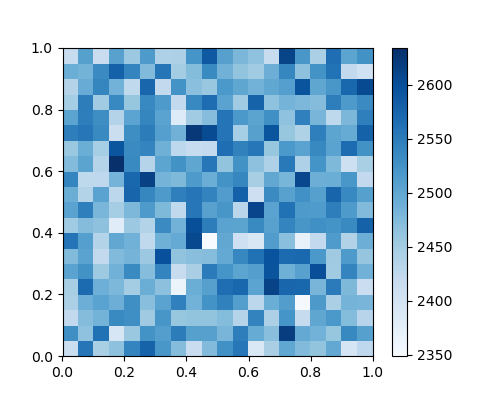
\includegraphics[height=6cm]{output/RNG_hist2d.png}
            \caption{The first thousand (left) and million (right) psuedo random numbers from the above generator. The coordinates of each point are given as  ($x_j$, $x_{j+1}$)}
            \label{fig:rng}
        \end{figure}
        


\end{document}
